\documentclass[]{article}
\usepackage{lmodern}
\usepackage{amssymb,amsmath}
\usepackage{ifxetex,ifluatex}
\usepackage{fixltx2e} % provides \textsubscript
\ifnum 0\ifxetex 1\fi\ifluatex 1\fi=0 % if pdftex
  \usepackage[T1]{fontenc}
  \usepackage[utf8]{inputenc}
\else % if luatex or xelatex
  \ifxetex
    \usepackage{mathspec}
  \else
    \usepackage{fontspec}
  \fi
  \defaultfontfeatures{Ligatures=TeX,Scale=MatchLowercase}
\fi
% use upquote if available, for straight quotes in verbatim environments
\IfFileExists{upquote.sty}{\usepackage{upquote}}{}
% use microtype if available
\IfFileExists{microtype.sty}{%
\usepackage[]{microtype}
\UseMicrotypeSet[protrusion]{basicmath} % disable protrusion for tt fonts
}{}
\PassOptionsToPackage{hyphens}{url} % url is loaded by hyperref
\usepackage[unicode=true]{hyperref}
\hypersetup{
            pdftitle={An Adapted Survey on Scientific Shared Resource Rigor and Reproducibility},
            pdfauthor={Add Your Name Here},
            pdfborder={0 0 0},
            breaklinks=true}
\urlstyle{same}  % don't use monospace font for urls
\usepackage[margin=1in]{geometry}
\usepackage{longtable,booktabs}
% Fix footnotes in tables (requires footnote package)
\IfFileExists{footnote.sty}{\usepackage{footnote}\makesavenoteenv{long table}}{}
\usepackage{graphicx,grffile}
\makeatletter
\def\maxwidth{\ifdim\Gin@nat@width>\linewidth\linewidth\else\Gin@nat@width\fi}
\def\maxheight{\ifdim\Gin@nat@height>\textheight\textheight\else\Gin@nat@height\fi}
\makeatother
% Scale images if necessary, so that they will not overflow the page
% margins by default, and it is still possible to overwrite the defaults
% using explicit options in \includegraphics[width, height, ...]{}
\setkeys{Gin}{width=\maxwidth,height=\maxheight,keepaspectratio}
\IfFileExists{parskip.sty}{%
\usepackage{parskip}
}{% else
\setlength{\parindent}{0pt}
\setlength{\parskip}{6pt plus 2pt minus 1pt}
}
\setlength{\emergencystretch}{3em}  % prevent overfull lines
\providecommand{\tightlist}{%
  \setlength{\itemsep}{0pt}\setlength{\parskip}{0pt}}
\setcounter{secnumdepth}{5}
% Redefines (sub)paragraphs to behave more like sections
\ifx\paragraph\undefined\else
\let\oldparagraph\paragraph
\renewcommand{\paragraph}[1]{\oldparagraph{#1}\mbox{}}
\fi
\ifx\subparagraph\undefined\else
\let\oldsubparagraph\subparagraph
\renewcommand{\subparagraph}[1]{\oldsubparagraph{#1}\mbox{}}
\fi

% set default figure placement to htbp
\makeatletter
\def\fps@figure{htbp}
\makeatother


\title{An Adapted Survey on Scientific Shared Resource Rigor and
Reproducibility}
\author{Add Your Name Here}
\date{December 15, 2020}

\begin{document}
\maketitle

\section{INTRODUCTION}\label{introduction}

\begin{quote}
\emph{``I have seen further it is because I have stood on the shoulders
of giants''} (Isaac Newton)
\end{quote}

Reproducible research practices include rigorously controlled and
documented experiments using validated reagents. These practices are
integral to the scientific method, and they enable acquisition of
reliable and actionable research results. However, the art and practice
of science is affected by challenges that go beyond the inherent
complexity of the biology being explored. The pressures to publish, the
focus on novel, positive, and impactful results, the use of suboptimal
research practices, and the scarcity of research funding likely
contribute to unacceptable levels of irreproducible scientific results
(Freedman, Venugopalan, \& Wisman, 2017).

A recent survey conducted by Springer (2016) reported that 90\% of
participants identified ``more robust experimental design'' as one of
several key improvements needed for the conduct of better science, in
addition to ``better statistics'' and ``better mentorship''. More
recently, Nature (2018) published the survey data which can be found on
Figshare.

A manifesto for reproducible science made several recommendations and
called attention to initiatives such as the \textbf{Transparency and
Openness Promotion} (TOP) guidelines created by the
\href{https://www.cos.io/}{Center for Open Science} to improve research
planning and reporting (Munafò, 2017), which was supported by over 5000
journals and research organizations.

On June 9, 2015, the U.S. National Institutes of Health (NIH) published
a notice\textsuperscript{1} that identified four areas for improvement
that are now required to be addressed by scientists in grant
applications, as follows:

\begin{enumerate}
\def\labelenumi{\arabic{enumi}.}
\item
  scientific premise forming the basis of the proposed research
\item
  rigorous experimental design for robust and unbiased results
\item
  consideration of sex and other relevant biologic variables
\item
  authentication of key biologic and chemical resources
\end{enumerate}

The \emph{Association of Biomolecular Resource Facilities} (ABRF)
\emph{Committee on Core Rigor and Reproducibility} (CCoRRe) recently
conducted a survey to assess how shared resource facilities are
currently assisting investigators with their need to demonstrate
transparency and rigor in their research. In addition, the survey
captured information from the shared resource personnel related to the
challenges they face and the resources they need to support scientific
transparency, rigor, and reproducibility.

\section{MATERIALS AND METHODS}\label{materials-and-methods}

\subsection{Survey Overview}\label{survey-overview}

The CCoRRe committee developed an 18-question online survey and shared
it using \href{https://surveymonkey.com}{SurveyMonkey}. The survey was
announced on the ABRF listservs and blogs and was open from February to
April 2017. All survey participants remained anonymous.

\subsection{Data Analysis}\label{data-analysis}

The survey contained both multiple-choice and open-ended text questions.
The open-ended text questions were categorized and coded following an
inductive coding approach with at least two independent coders. Using
the sampling error formula

\[ e = { Zp(1-p) \over \sqrt{n} } \]

we compute that at a 95\% confidence level (i.e., \(Z=1.96\)), with base
probability \(p=1/2\) and sample size \(n=243\), the margin of error is
±3\%.

\section{RESULTS AND DISCUSSION}\label{results-and-discussion}

\subsection{Survey Demographics}\label{survey-demographics}

A total of 243 individuals from 21 countries completed this section. The
majority of the survey participants are core facility directors or
managers (69\%) and work in an academic setting (72\%) in the United
States (79\%).

\subsection{Current Landscape for Rigor and Transparency in Represented
Shared
Resources}\label{current-landscape-for-rigor-and-transparency-in-represented-shared-resources}

When asked how knowledgeable participants were with respect to the NIH
research rigor initiatives, 47\% stated they were very familiar, whereas
the rest were equally either somewhat familiar or completely unaware of
such guidelines (Fig. 1).

\begin{figure}
\centering
\includegraphics{C:/Users/twhite/Documents/Github/R-markdown/paperToRmd/code/../results/Paper_Template_html_files/figure-latex/unnamed-chunk-2-1.pdf}
\caption{FIGURE 1 - Knowledge and awareness of the current NIH
guidelines on rigor and reproducibility.}
\end{figure}

Time pressures associated with publishing and grant preparation were
frequently identified as risks to research rigor. Many respondents noted
that inadequate standardization of protocols and procedures across the
research life cycle, from study planning through data analysis and
reporting, contributes to variable research quality. As previously
reported, (Bustin, 2014; Freedman et al., 2017) respondents indicated
that experimental design deficiencies (involving sample size, quality
control, and replication) and cost considerations could generate risks
to research rigor and transparency.

Table 1 represents the perceived challenges faced in promoting best
practices for rigorous research in core settings. Issues associated with
sample quality or quantity top the list.

TABLE 1 - Major challenges to rigor observed in shared resources

\begin{longtable}[]{@{}ll@{}}
\toprule
\begin{minipage}[b]{0.05\columnwidth}\raggedright\strut
\textbf{Category}\strut
\end{minipage} & \begin{minipage}[b]{0.05\columnwidth}\raggedright\strut
\textbf{N}\strut
\end{minipage}\tabularnewline
\midrule
\endhead
\begin{minipage}[t]{0.05\columnwidth}\raggedright\strut
Poor sample quality from users/sample variability/limited biological
material\strut
\end{minipage} & \begin{minipage}[t]{0.05\columnwidth}\raggedright\strut
51\strut
\end{minipage}\tabularnewline
\begin{minipage}[t]{0.05\columnwidth}\raggedright\strut
Lack of well-trained principle investigators and lab members/Poor
oversight\strut
\end{minipage} & \begin{minipage}[t]{0.05\columnwidth}\raggedright\strut
45\strut
\end{minipage}\tabularnewline
\begin{minipage}[t]{0.05\columnwidth}\raggedright\strut
Poor experimental design: Lack of sufficient replicates/inadequate
sample size/lack of adequate controls\strut
\end{minipage} & \begin{minipage}[t]{0.05\columnwidth}\raggedright\strut
43\strut
\end{minipage}\tabularnewline
\begin{minipage}[t]{0.05\columnwidth}\raggedright\strut
Inadequate standardization of protocols or guidelines, and data
analysis\strut
\end{minipage} & \begin{minipage}[t]{0.05\columnwidth}\raggedright\strut
43\strut
\end{minipage}\tabularnewline
\begin{minipage}[t]{0.05\columnwidth}\raggedright\strut
Cost and time\strut
\end{minipage} & \begin{minipage}[t]{0.05\columnwidth}\raggedright\strut
39\strut
\end{minipage}\tabularnewline
\begin{minipage}[t]{0.05\columnwidth}\raggedright\strut
Failure to leverage the core's expertise/following the core's advice/no
consulting beforehand\strut
\end{minipage} & \begin{minipage}[t]{0.05\columnwidth}\raggedright\strut
23\strut
\end{minipage}\tabularnewline
\begin{minipage}[t]{0.05\columnwidth}\raggedright\strut
Inadequate documentation of experiments/data management\strut
\end{minipage} & \begin{minipage}[t]{0.05\columnwidth}\raggedright\strut
19\strut
\end{minipage}\tabularnewline
\begin{minipage}[t]{0.05\columnwidth}\raggedright\strut
Instruments: maintenance, upgrades, changes\strut
\end{minipage} & \begin{minipage}[t]{0.05\columnwidth}\raggedright\strut
15\strut
\end{minipage}\tabularnewline
\begin{minipage}[t]{0.05\columnwidth}\raggedright\strut
Responses that could not be assigned to a category\strut
\end{minipage} & \begin{minipage}[t]{0.05\columnwidth}\raggedright\strut
11\strut
\end{minipage}\tabularnewline
\bottomrule
\end{longtable}

Just over 70\% of respondents noted that their clients do not routinely
request specific information (documentation or practice statements)
related to the procedures used by the cores to foster rigorous and
reproducible research (Fig. 2).

\begin{figure}
\centering
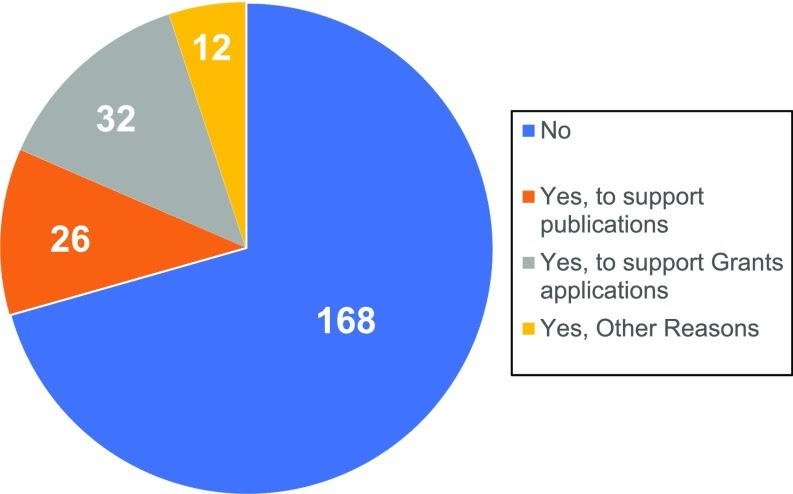
\includegraphics[width=0.50000\textwidth,height=0.50000\textwidth]{../figs/fig2_paper.jpg}
\caption{FIGURE 2 - Lack of requests for rigor and reproducibility
documentation by users of shared resources.}
\end{figure}

The apparent lack of core engagement at the institutional level does not
necessarily reflect a general lack of rigor in the daily operations of
the cores. Indeed, 213 out of 216 who participated in this section of
the survey selected at least one tool that they currently use to support
R\&R in their daily core operations and almost 75\% indicated at least
four more tools. With that regard, it is important to highlight:

\begin{itemize}
\tightlist
\item
  At least 170 (∼80\%) respondents use documentation, in the form of
  quality control and standard operation procedures (SOPs) to support
  R\&R practices.
\item
  The incorporation of an instrumentation management plan, was not as
  highly utilized (56\%).
\item
  Oversight of data analyses and double-checking results were some of
  the least widely used ones (26\%).
\end{itemize}

A second set of multiple-choice questions asked participants to select
the new tools they think would enhance or facilitate the implementation
of R\&R best practices within their core operation (Fig. 3).

\begin{figure}
\centering
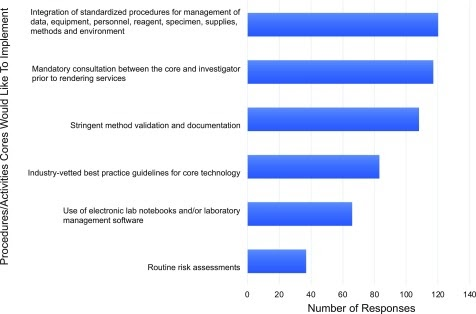
\includegraphics[width=0.60000\textwidth,height=0.80000\textwidth]{../figs/fig3_paper.jpg}
\caption{FIGURE 3 - Types of tools that cores would like to implement in
their operations.}
\end{figure}

\subsection{Core Implementation of Research Best
Practices}\label{core-implementation-of-research-best-practices}

Optimal research core services require a full commitment to rigorous
methods as an obligation and not as a choice. However, more than half of
the participants identified lack of funding and technical staff training
as primary deterrents to the implementation and maintenance of R\&R
initiatives. This illustrates the difficulties that fee-for-service core
facilities face when considering the costs associated with establishing
new standardized procedures, methods, or technologies, or improving
documentation, transparency, and quality control.

\subsection{Strategies for Improving R\&R in Core
Operation}\label{strategies-for-improving-rr-in-core-operation}

Participants were asked to suggest solutions to mitigate or eliminate
challenges and provide a clear path to improved R\&R in cores. Some of
the responders did emphasize the need for the development of universal
guidelines and SOPs that would facilitate the consistent adoption across
a technology or application and would incentivize investigators to
comply with such published R\&R guidelines.

About 40\% proposed that funding mechanisms should be available to cores
from either discretionary institutional funds or federal agencies to
promote and support R\&R initiatives. It is clear that survey
respondents believe that it is important to identify funding mechanisms
to help core service providers become more visible as scientific
experts, partners, and educators with the ability to directly influence
research quality.

About one quarter of respondents noted that a radical cultural change at
the highest institutional levels is necessary to support and foster
research rigor and transparency. Research institutions, journals, and
funding agencies must be willing to establish clear requirements as well
as mandate and ``provide incentives to support and monitor research
rigor throughout the research life cycle'' These ``cultural''
observations related to research culture and incentives were frequently
noted in previously published reviews of the research reproducibility
issue (Baker, 2016; Freedman et al., 2017).

\section{CONCLUSIONS}\label{conclusions}

Scientific shared resources support research laboratories to generate
critical data across many disciplines. Core personnel maintain
considerable expertise that is important for the quality of their work
and for sharing with research scientists in their important role as
research mentors. They ensure continuous improvement through
professional and educational development and through their systematic
approach to research methods.

\textsuperscript{1}Through these four elements, the NIH intends to
``enhance the reproducibility of research findings through increased
scientific rigor and transparency''
(\url{https://ori.hhs.gov/images/ddblock/ORI\%20Data\%20Graphs\%202006-2015.pdf})

\section*{REFERENCES}\label{references}
\addcontentsline{toc}{section}{REFERENCES}

\hypertarget{refs}{}
\hypertarget{ref-baker_1500_2016}{}
Baker, M. (2016). 1,500 scientists lift the lid on reproducibility.
\emph{Nature News}, \emph{533}(7604), 452. Retrieved November 13, 2020,
from
\url{http://www.nature.com/news/1-500-scientists-lift-the-lid-on-reproducibility-1.19970}

\hypertarget{ref-bustin_reproducibility_2014}{}
Bustin, S. A. (2014). The reproducibility of biomedical research:
Sleepers awake! \emph{Biomolecular Detection and Quantification},
\emph{2}, 35--42. Retrieved November 13, 2020, from
\url{http://www.sciencedirect.com/science/article/pii/S2214753515000030}

\hypertarget{ref-freedman_reproducibility2020_2017}{}
Freedman, P., Venugopalan, G., \& Wisman, R. (2017).
Reproducibility2020: Progress and priorities. \emph{F1000Research},
\emph{6}. Retrieved November 13, 2020, from
\url{https://www.ncbi.nlm.nih.gov/pmc/articles/PMC5461896/}

\hypertarget{ref-munafo_manifesto_2017}{}
Munafò, M. R. et a. (2017). A manifesto for reproducible science.
\emph{Nature Human Behaviour}, \emph{1}(1), 1--9. Retrieved November 13,
2020, from \url{https://www.nature.com/articles/s41562-016-0021}

\hypertarget{ref-nature_nature_2018}{}
Nature. (2018). Nature Reproducibility survey 2017. \emph{Figshare}.
Repository,. Retrieved from \url{10.6084/m9.figshare.6139937.v4}

\hypertarget{ref-springer_reality_2016}{}
Springer, N. (2016). Reality check on reproducibility. \emph{Nature},
\emph{533}(7604), 437.

\end{document}
